% $RCSfile$
% $Revision$
% $Date$
% $Source$
%
%
% ---------------------------------------------------------------------------
% TODO:
%
% FINAL READ 
% - check for consistent tense
% - query replace: ai2tv -> $\mathrm{AI}^2$TV
% - spell check
%
%
% ---------------------------------------------------------------------------
% This is "sig-alternate.tex" V1.3 OCTOBER 2002
% This file should be compiled with V1.6 of "sig-alternate.cls" OCTOBER 2002
%
% This example file demonstrates the use of the 'sig-alternate.cls'
% V1.6 LaTeX2e document class file. It is for those submitting
% articles to ACM Conference Proceedings WHO DO NOT WISH TO
% STRICTLY ADHERE TO THE SIGS (PUBS-BOARD-ENDORSED) STYLE.
% The 'sig-alternate.cls' file will produce a similar-looking,
% albeit, 'tighter' paper resulting in, invariably, fewer pages.
%
% ---------------------------------------------------------------------------
% This .tex file (and associated .cls V1.6) produces:
%       1) The Permission Statement
%       2) The Conference (location) Info information
%       3) The Copyright Line with ACM data
%       4) NO page numbers
%
% as against the acm_proc_article-sp.cls file which
% DOES NOT produce 1) thru' 3) above.
%
% Using 'sig-alternate.cls' you have control, however, from within
% the source .tex file, over both the CopyrightYear
% (defaulted to 2002) and the ACM Copyright Data
% (defaulted to X-XXXXX-XX-X/XX/XX).
% e.g.
% \CopyrightYear{2003} will cause 2002 to appear in the copyright line.
% \crdata{0-12345-67-8/90/12} will cause 0-12345-67-8/90/12 to appear in the
%  copyright line.
%
% ---------------------------------------------------------------------------
% This .tex source is an example which *does* use
% the .bib file (from which the .bbl file % is produced).
% REMEMBER HOWEVER: After having produced the .bbl file,
% and prior to final submission, you *NEED* to 'insert'
% your .bbl file into your source .tex file so as to provide
% ONE 'self-contained' source file.
%
% ================= IF YOU HAVE QUESTIONS =======================
% Questions regarding the SIGS styles, SIGS policies and
% procedures, Conferences etc. should be sent to
% Adrienne Griscti (griscti@acm.org)
%
% Technical questions _only_ to
% Gerald Murray (murray@acm.org)
% ===============================================================
%
% For tracking purposes - this is V1.3 - OCTOBER 2002
\documentclass{sig-alternate}
\usepackage{url}

\begin{document}

%
% --- Author Metadata here ---
\conferenceinfo{ACM-MM 2004}{New York, NY USA}
%\CopyrightYear{2001}
% Allows default copyright year (2000) to be over-ridden - IF NEED BE.

%\crdata{0-12345-67-8/90/01}
% Allows default copyright data (0-89791-88-6/97/05) to be over-ridden - IF NEED BE.
% --- End of Author Metadata ---

% \title{Optimizing Quality for Video Sharing in Synchronous Collaboration}
\title{Optimizing Quality for Collaborative Video Viewing}
%
% You need the command \numberofauthors to handle the "boxing"
% and alignment of the authors under the title, and to add
% a section for authors number 4 through n.
%
% Up to the first three authors are aligned under the title;
% use the \alignauthor commands below to handle those names
% and affiliations. Add names, affiliations, addresses for
% additional authors as the argument to \additionalauthors;
% these will be set for you without further effort on your
% part as the last section in the body of your article BEFORE
% References or any Appendices.

\numberofauthors{4}
%
% You can go ahead and credit authors number 4+ here;
% their names will appear in a section called
% "Additional Authors" just before the Appendices
% (if there are any) or Bibliography (if there
% aren't)

% Put no more than the first THREE authors in the \author command
\author{
%
% The command \alignauthor (no curly braces needed) should
% precede each author name, affiliation/snail-mail address and
% e-mail address. Additionally, tag each line of
% affiliation/address with \affaddr, and tag the
%% e-mail address with \email.
\alignauthor Dan Phung\\
       \affaddr{Computer Science Department}\\
       \affaddr{Columbia University}\\
       \affaddr{New York City, New York}\\
       \email{phung@cs.columbia.edu}
\alignauthor Giuseppe Valetto\\
       \affaddr{Computer Science Department}\\
       \affaddr{Columbia University}\\
       \affaddr{New York City, New York}\\
       \affaddr{and Telecom Italia Lab}\\
       \affaddr{Turin, Italy}
       \email{valetto@cs.columbia.edu}
\alignauthor Gail Kaiser \\
       \affaddr{Computer Science Department}\\
       \affaddr{Columbia University}\\
       \affaddr{New York City, New York}\\
       \email{kaiser@cs.columbia.edu}
}
\additionalauthors{Additional authors: Suhit Gupta {\texttt{suhit@columbia.cs.edu}}}
\date{\parbox[b][0ex]{0em}{\hspace*{-12.5em}\raisebox{37ex}{\fbox{For
submission to \emph{ACM-MM 2004}, due 12:00 AM EDT: April 05, 2004.}}}}
% \date{05 April 2004}
\maketitle

\begin{abstract}
The increasing popularity of distance learning and online courses has
highlighted the lack of collaborative tools for student groups.  In
addition, the introduction of lecture videos into the online
curriculum has drawn attention to the disparity in the network
resources used by the students.  We present an architecture and
adaptation model called $\mathrm{AI}^2$TV (Adaptive Internet
Interactive Team Video), a system that allows geographically dispersed
participants, possibly some or all disadvantaged in network resources,
to collaboratively view a video in synchrony.  $\mathrm{AI}^2$TV
upholds the invariant that each participant will view semantically
equivalent content at all times. Video player actions, like play,
pause and stop, can be initiated by any of the participants and the
results of those actions are seen by all the members.  These features
allow group members to review a lecture video in tandem to facilitate
the learning process.  We employ an autonomic (feedback loop)
controller that monitors clients' video status and adjusts the quality
of the video according to the resources of each client.  We show in
experimental trials that our system can successfully synchronize video
for distributed clients while at the same time optimizing the video
quality, given actual (fluctuating) bandwidth, by adaptively adjusting
the quality level for each participant.
\end{abstract}

% A category with the (minimum) three required fields
\category{C.2.4}{Distributed Systems}{Client/server, Distributed applications}
\category{D.2.8}{Software Engineering}{Metrics -- performance measures}
\category{H.5.1}{Information Interfaces and Presentation}{Multimedia Information Systems}
\category{H.5.3}{\\Group and Organization Interfaces}{Computer-\\supported cooperative work, Synchronous interaction}
\category{K.3.1}{Computer Uses In Education}{Collaborative learning, Distance learning}

\terms{ALGORITHMS, MEASUREMENT, PERFORMANCE, EXPERIMENTATION, HUMAN
FACTORS}

\keywords{Synchronized Collaborative Video, Autonomic Controller}

% -------------------------------------------------- %
% FIGURES AT THE FRONT
% -------------------------------------------------- %
%% \begin{figure}
%%   \centering
%%   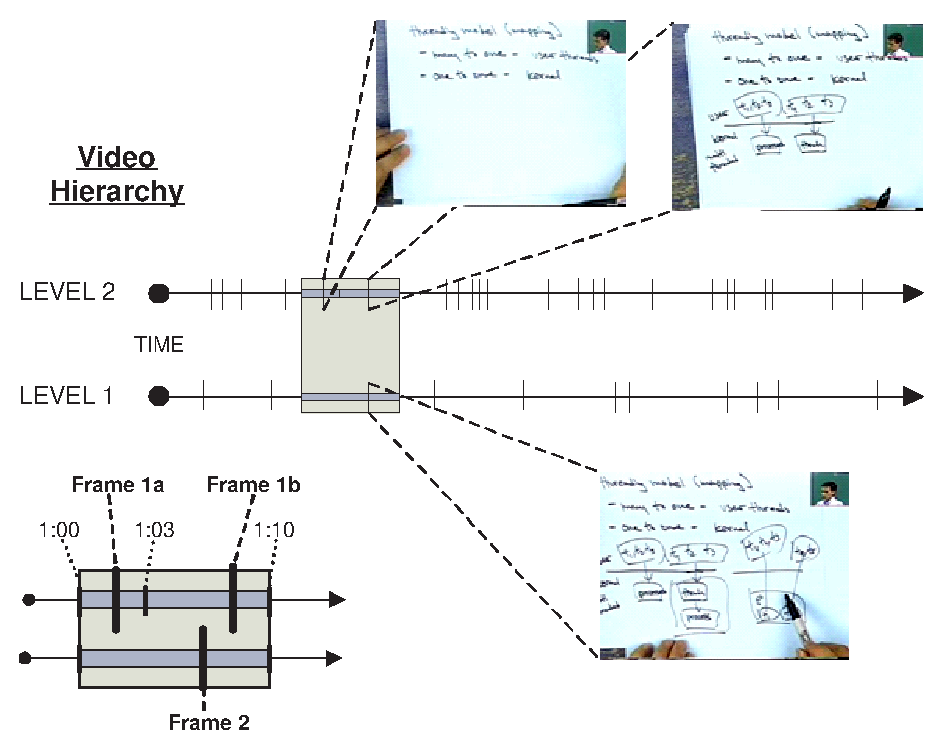
\epsfig{file=vidframes.eps, width=8cm}
%%   \caption{Semantic video compression hierarchy.}
%%   \label{vidframes}
%% \end{figure} 

%% \begin{figure}
%%   \centering
%%   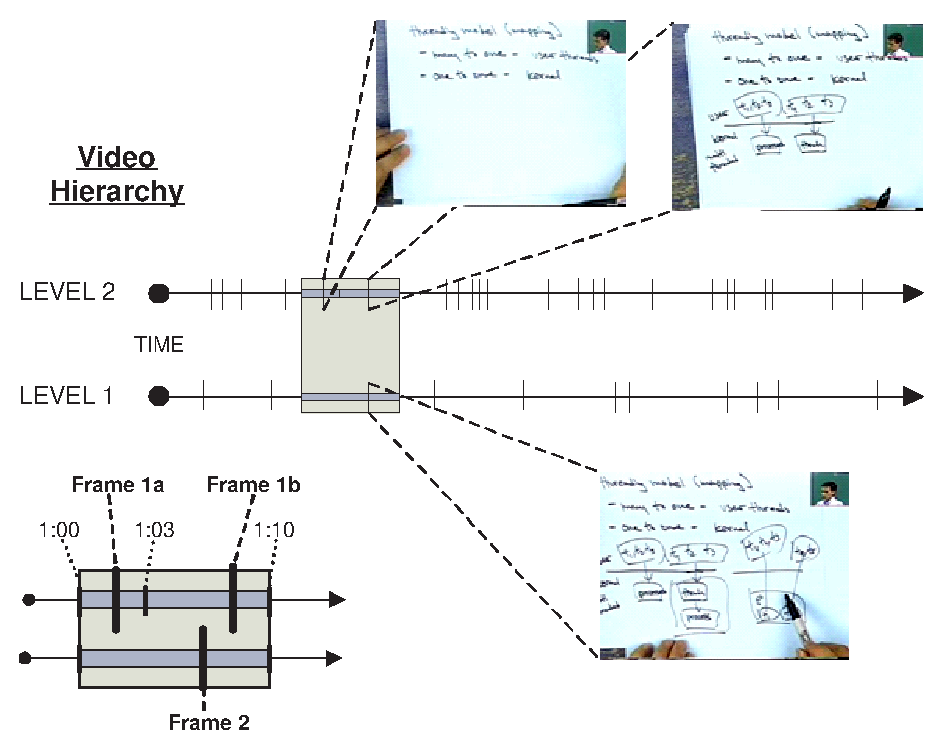
\epsfig{file=vidframes.eps, width=8cm}
%%   \caption{Semantic video compression hierarchy.}
%%   \label{vidframes}
%% \end{figure} 

%% \begin{figure}
%%   \centering
%%   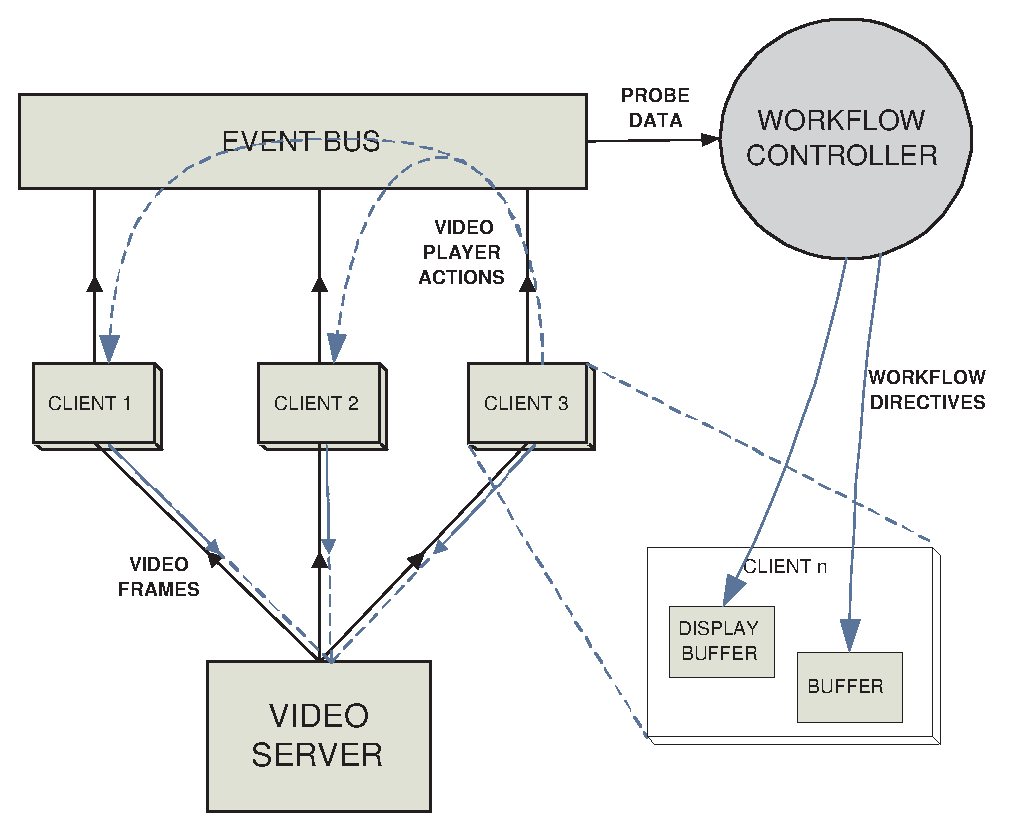
\epsfig{file=ai2tvarch.eps, width=8cm}
%%   \caption{ai2tv Architecture}
%%   \label{ai2tv_arch}
%% \end{figure}


%% \begin{figure}
%%  \centering
%%  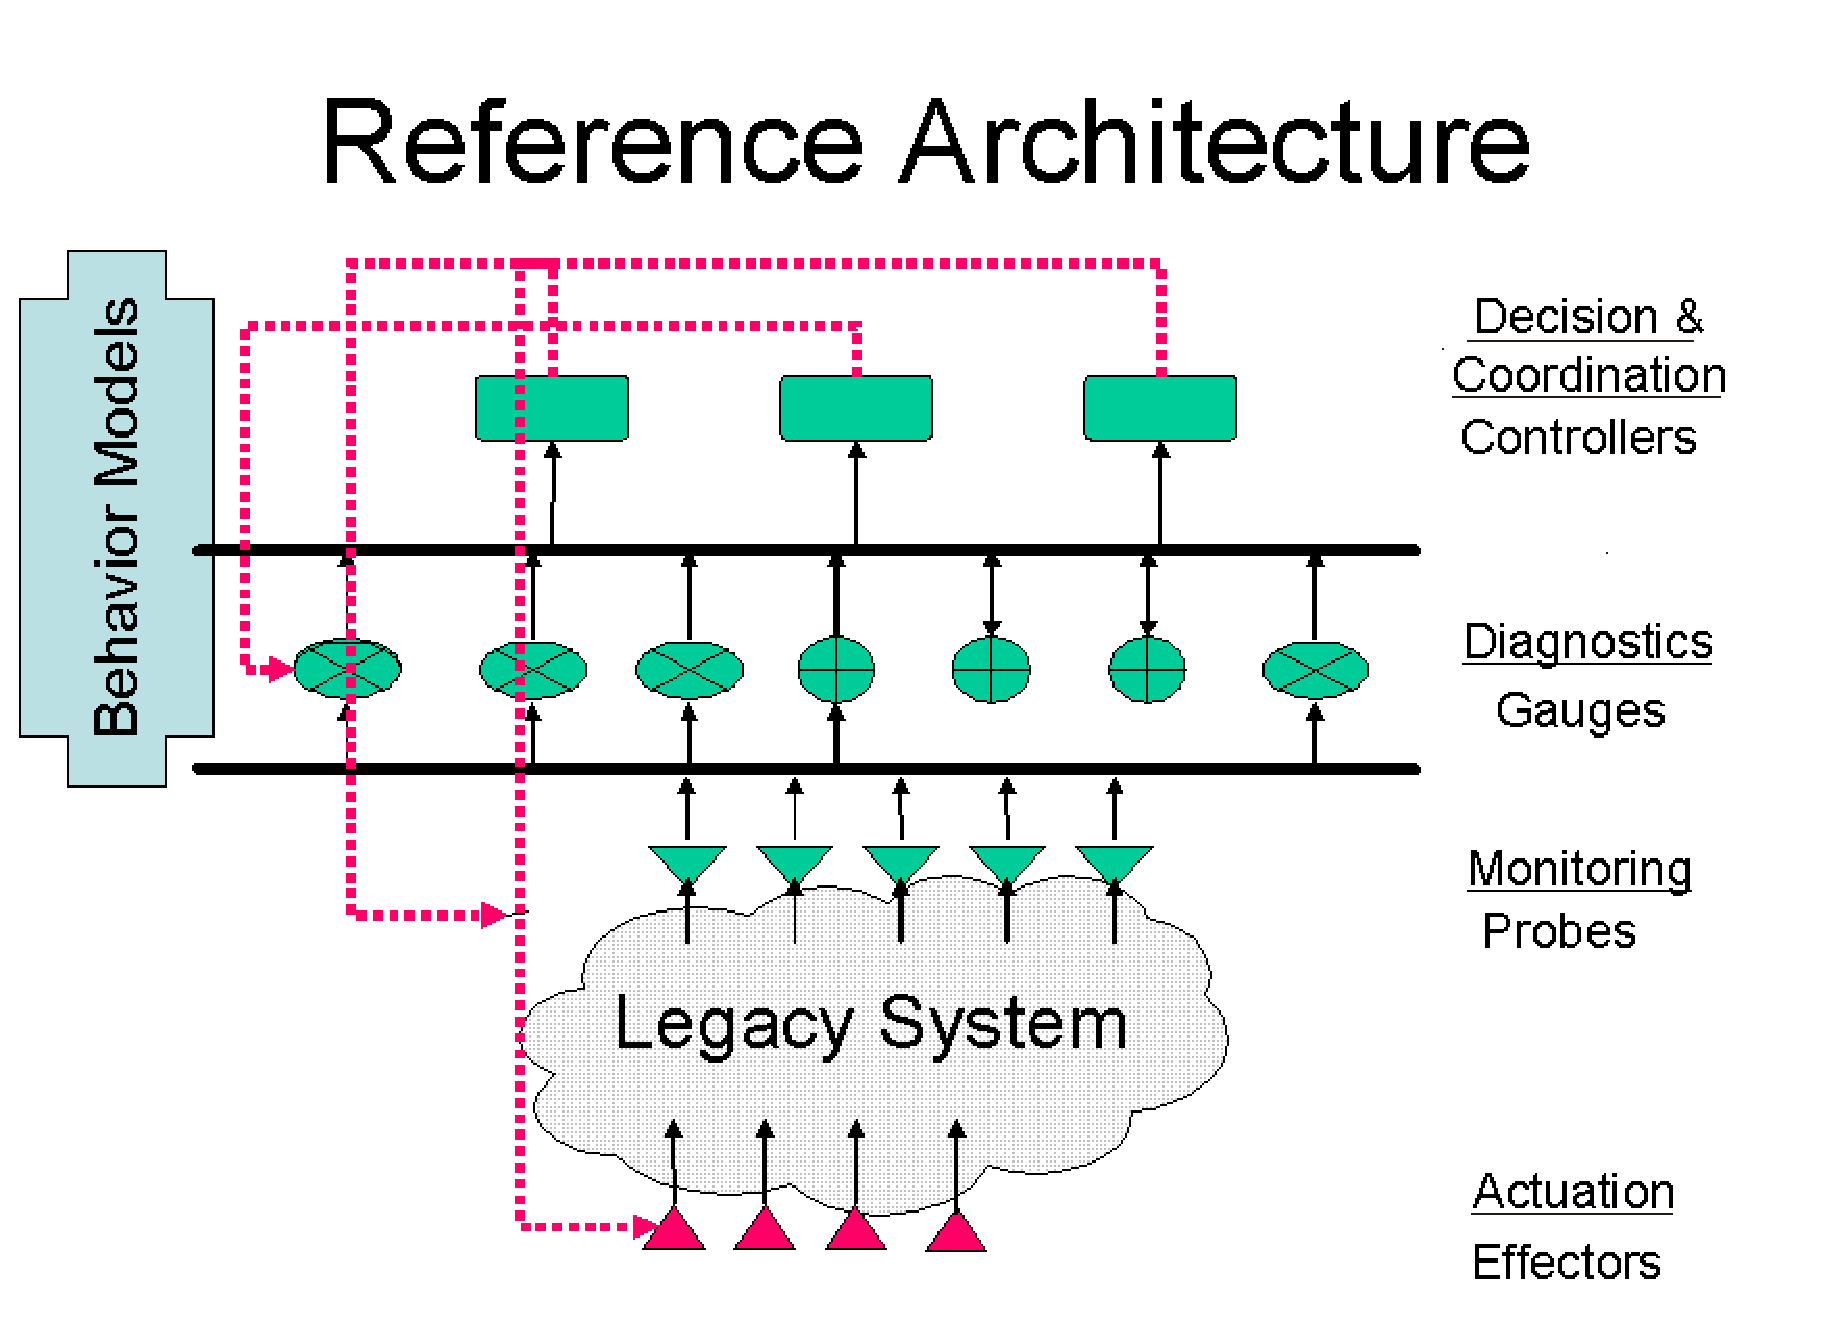
\epsfig{file=refarch.eps, width=8cm}
%%   \label{refarch}
%%  \caption{Conceptual Reference Architecture}
%% \end{figure}


%% \begin{figure} 
%%   \centering
%%   \hspace*{-5mm}
%%   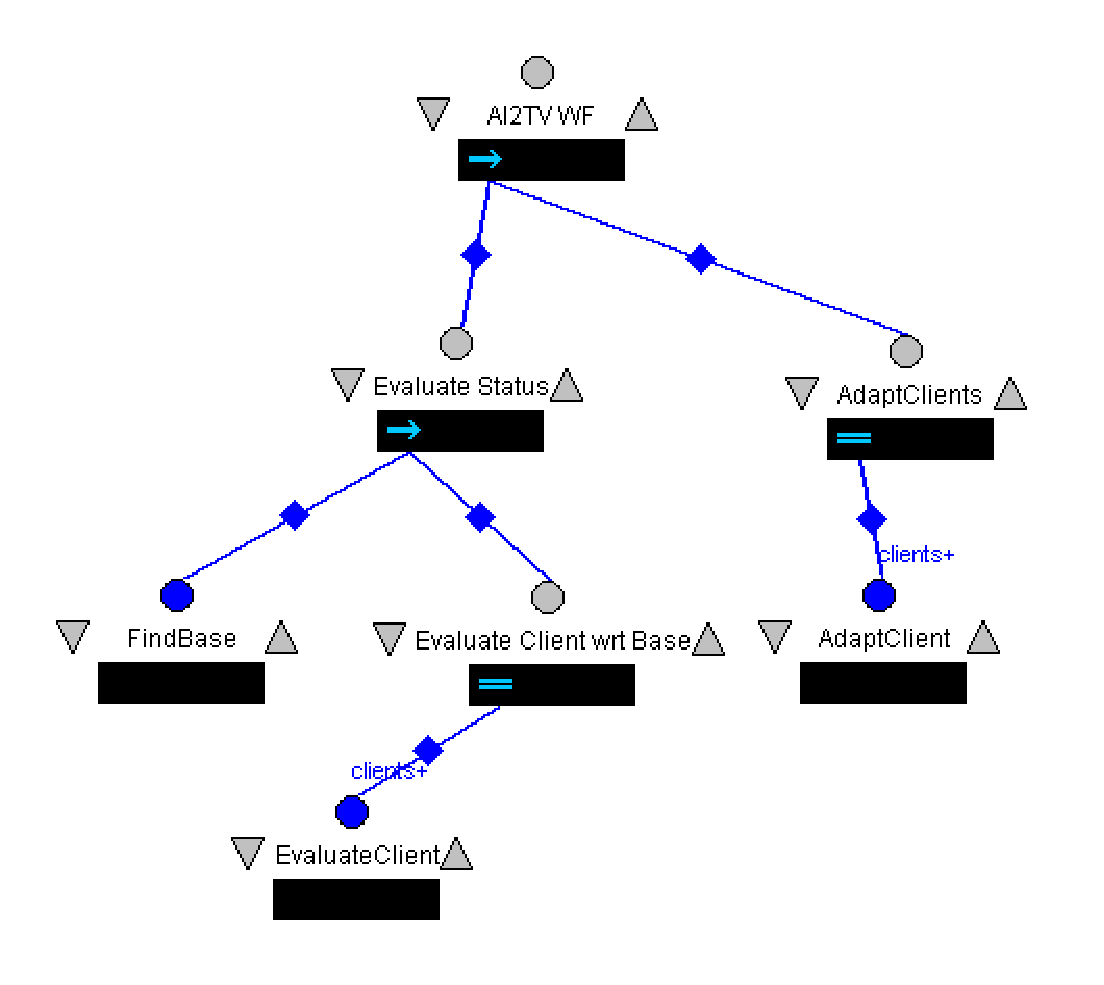
\epsfig{file=ljil.eps, width=8cm}
%%   \caption{Workflow diagram }
%%   \label{ljil}
%% \end{figure}


% -------------------------------------------------- %

% tech report number CUCS-009-04
\section{Introduction}

% The wording was awkward here, so I pretend that Stanford also
% once fedexed, even tho we don't know that.  

% Dan - you didn't insert any of the original cites into the new
% Introduction, weren't any of them relevant?

Distance learning programs such as the Columbia Video Network and the
Stanford Center for Professional Development have evolved from
fedexing lecture video tapes to their off-campus students to instead
streaming the videos over the Internet.  The lectures might be
delivered ``live'', while in progress on campus, but are frequently
post-processed and packaged for students to watch (and re-watch) at
their convenience.  This introduces the possibility of forming ``study
groups'' among off-campus students who view the lecture videos
together, and pause the video for discussion when desired, thus
approximating the pedagogically valuable discussions of on-campus
students.  Although the instructor is probably not available for these
discussions, this may be an advantage, since on-campus students are
rarely afforded the opportunity to pause, rewind and fast-forward
their instructors' lectures.

% should it be JPG or JPEG?

However, what we call {\em collaborative video viewing} by multiple
geographically dispersed users is not yet supported by conventional
Internet-video technology.  It is particularly challenging to support
WISIWYS (what I see is what you see) when some of the users are
relatively disadvantaged with respect to bandwidth (e.g., dial-up
modems) and local computer resources (e.g., archaic graphics cards,
small disks).  We have adopted technology (developed by others, Liu
and Kender \cite{TIECHENG}) for ``semantically compressing'' standard
MPEG videos into sequences of still JPEG images.  This technology
automatically selects the most semantically meaningful frames to show
for each time epoch, and can generate different sequences of JPEG
images for a range of different compression (bandwidth) levels.  This
approach works very well for typical lecture videos, where it is
important, for instance, to see what the instructor has written on the
blackboard after he/she stands aside, but probably not so important to
see the instructor actually doing the writing, when his/her hand and
body may partially occlude the blackboard.

The remaining technical challenge is {\em synchronizing} the
downloading and display of the image sequences among each of the
distributed user clients, including support for shared video player
actions such as pause, rewind, etc.  Further, if student groups do
indeed sometimes pause the videos, or rewind to a point already
available in local buffers (caches), it is desirable to take advantage
of the then-idle network connection to prefetch future images at a
higher quality level.

% cite for NTP?

We have developed an approach to achieving this, using three
mechanisms working in tandem.  First, the software clocks of the video
clients are synchronized using NTP.  This time is used for reference
within the image sequences, where each image is associated with its
start and end times relative to the beginning of the sequence.
Second, the video clients communicate with each other over a
distributed publish-subscribe event bus, which propagates video
actions taken by one user in the group to all the other users in the
group.  Thus any user can select a video action, not just a
``leader''.

Finally, the main innovation of this research concerns optimizing
video quality in this context: A decentralized feedback control loop
dynamically adjusts each video client's choice of both next image to
display and also next image to retrieve from the semantic compression
levels available.  The controller relies on sensors embedded in each
client to periodically check what image is currently displaying,
whether this image is ``correct'' for the current NTP time compared to
what other clients are viewing, which images have already been
buffered (cached) at that client, and what is the actual bandwidth
recently perceived at that client.  Actuators are also inserted into
the video clients, to modify local configuration parameters on
controller command. The controller utilizes detailed information about
the image sequences available at the video server, including image
start and stop times (both the individual images and their start and
stop times tend to be different at different compression levels), but
unlike local client data, video server data is unlikely to change
while the video is showing.  A single controller is used for all
clients in the same user group, so it can detect ``skew'' across
multiple clients, and may reside on the video server or on another
host on the Internet.

In the next section, we further motivate the collaborative video
viewing problem, provide background on the semantically compressed
video repository, and explain the technical difficulties of optimizing
quality while synchronizing such semantically compressed videos. The
following section presents our architecture and dynamic adaptation
model, and its implementation in $\mathrm{AI}^2$TV (Adaptive
Interactive Internet Team Video).  In the Evaluation section, we
describe the criteria used to evaluate the effectiveness of our
approach, and show empirical results obtained when applied to real
lecture videos distributed for a recent Columbia Video Network
course. We compare to related work, and then summarize our
contributions.

\section{Motivation and Background} \label{background}

% - discuss other projects on multiple client synchronization 
% shouldn't that go in the related work section?

Correspondence courses have been available to working adult and/or
geographically remote learners for over a century, e.g., the American
School in Illinois has offered high school courses since 1897
\cite{AmericanSchool}, and the University of Wyoming began offering
extension courses in 1892, launching a full-fledged college distance
learning program in 1906 \cite{UWyoming}.  Correspondence courses have
traditionally been designed for individual students with a
self-motivated learning style, studying primarily from reading
materials and possibly text ``lectures''.

% would be good if a cite could be found for last sentence above

An NSF Report \cite{NSFReport} discusses how technology, from radio to
television, to audio and video cassettes, to audio and video
conferencing, has affected distance education. These technologies have
enabled universities to offer certification and degree tracks using
live or pre-taped audio and/or video of regular on-campus classroom
lectures.  The report states that the recent use of Internet
technologies, especially the Web, has ``allowed both synchronous and
asynchronous communication among students and between faculty and
students'' and has ``stimulated renewed interest in distance
education''. It also mentions that ``stimulating interaction among
students'' can help reduce dropout rates, which may be higher in
distance education than in traditional courses. Finally, it cites some
studies that ``suggest the Web is superior to earlier distance
education technologies because it allows teachers to build
collaborative and team-oriented communities rather than either the
passive classes of the conventional academy or the individual study of
traditional correspondence courses''.

Today's equivalent of correspondence courses are often offered online
through a Web portal interface, with some for-profit schools like
University of Phoenix \cite{UPhoenix} and Capella University
\cite{Capella} primarily online.  Tools such as instant messaging,
application and desktop sharing \cite{WEBEX, VNC}, and co-browsing
\cite{CAPPS, LIEBERMAN, SIDLER} facilitate the communicative aspects
of synchronous collaboration but are not designed specifically for
educational purposes.  Support for synchronous collaboration remains a
major concern in courses where group work is encouraged \cite{WELLS},
yet there are few educational tools that allow synchronous
collaboration across a group of online students \cite{BURGESS}.
However, it seems that Web-based video streaming should enable
synchronous collaboration ``situated'' by collaborative lecture video
viewing.

% would be good to find a cite for the last sentence above

% - ai2tv project goals

Our $\mathrm{AI}^2$TV project aims to contribute to the area of
synchronous collaboration support for distance education, specifically
in the context of collaborative video viewing over the Internet.

Viewing video on the Internet usually requires relatively high
bandwidth resources, and low-bandwidth or lossy network connections
can lead to lost video content.  This is particularly a problem for
group review of lecture videos, if different members of the group miss
different portions of the video or fall behind to different degrees
due to extensive buffering.  Furthermore, the differences in network
and computing resources available to dispersed users may make it
difficult -- with current video technology -- for some students to
participate in collaborative video viewing at all.  

Technically, collaborative video sharing poses a twofold problem: on
the one hand, it is mandatory to keep all users synchronized with
respect to the content they are supposed to see at any moment during
play time; on the other hand, it is important to provide each
individual user with a frame rate that is optimized with respect to
the user's available resources, which may vary during the course of
the video.

One solution to the problem of balancing the group synchronization
requirement with the optimization of individual viewing experiences is
to use videos with cumulative layering \cite{MCCANNE}, also known as
scalable coding \cite{LI}.  In this approach, the client video player
selects a quality level appropriate for that client's resources from a
hierarchy of several different encodings or frame rates for that
video. Thus a client could receive an appropriate quality of video
content while staying in sync with the other members of the group.

% so why isn't the above approach good enough, do we do better?

% - describe overview of semantic compression tool used

In $\mathrm{AI}^2$TV, we use {\em semantic summarization} to produce a
video with cumulative layering.  A semantic summarization algorithm
and corresponding software package developed here at Columbia by Liu
and Kender \cite{TIECHENG} reduces a video to a set of semantically
significant key frames.  That tool operates on conventional MPEG
format videos and outputs sequences of JEPG frames, some of which are
displayed in figure \ref{sem_video}.  The semantic summarization (or
semantic compression) algorithm profiles video frames within a sliding
time window and selects key frames that have the most semantic
information with respect to that window.  By increasing the size of
the window, a key frame will represent a larger time slice, which
means that a larger window size will produce less key frames as
compared to a smaller window size setting.

\begin{figure}
  \centering
  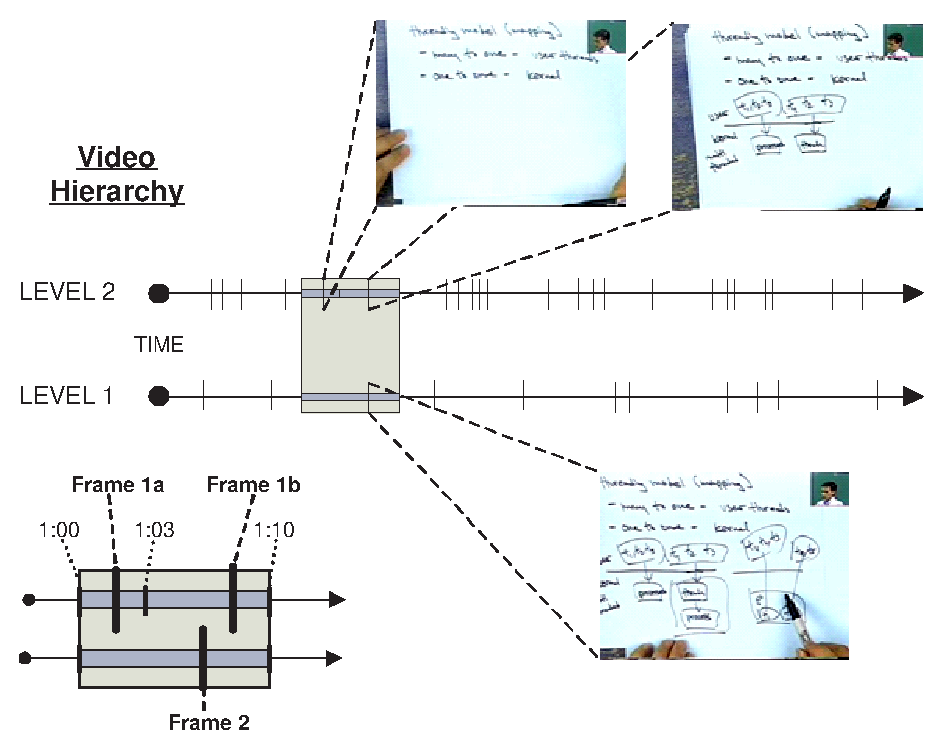
\epsfig{file=vidframes.eps, width=8cm}
  \caption{Semantic Video Scenario}
  \label{sem_video}
\end{figure} 

A conceptual diagram of a layered video produced from this semantic
compression is shown in figure \ref{sem_video}.  Note that the
semantic compression algorithm produces an effectively random
distribution of key frames, hence the video produced by the package
plays back at a {\em variable} frame rate.  The variability in the
frame rate is most significant when there are pockets of relatively
high frequency semantic change, which result in sections in the video
that demand a higher frame rate.  The variable frame rate video adds
substantial complexity to the bandwidth demands of the client.

Also, in figure \ref{sem_video}, the bottom-left in-set shows the
juxtaposition of individual frames from two different quality levels.
Each frame has a representative time interval \texttt{[start:end]}.
For the higher level, Frame 1a represents the interval from 1:00 to
1:03, and Frame 1b represents the interval from 1:04 to 1:10.  For the
lower level, Frame 2 represents the entire interval from 1:00 to 1:10.
In this diagram, Frame 2 is semantically equivalent to Frame 1a and 1b
together.  However, in real JPEG frame sequences produced from the
same MPEG video for different quality levels, the start and end times
of frame sets rarely match up as ideally as in our example.

Through the use of the Liu/Kender video compression algorithm, we can
potentially provide semantically equivalent content to a group of user
clients with diverse resources by adjusting the compression level
assigned to each client while the users are watching the video.  Thus
for our purposes, synchronization of collaborative video boils down to
showing semantically equivalent frames.

To adjust the clients in response to the changing environment, we use
an ``autonomic'' controller to maintain the synchronization of the
group of video clients while simultaneously fine tuning the video
quality for each client.  The term \textit{autonomic} is borrowed from
IBM to mean a self-managing system that uses a (software) feedback
control loop \cite{IBM}.  Their terminology was invented for the
self-management of data center operations, whereas our application
applies to the relatively novel domain of multi-user video
synchronization.  

Our autonomic controller remains conceptually separate from the
controlled $\mathrm{AI}^2$TV video system, employing our decentralized
workflow engine, named Workflakes \cite{ValettoThesis}, to achieve the
control capabilities.  Said workflow coordinates the behavior of
software entities, as opposed to conventional human-oriented workflow
systems; the use of workflow technology for the specification and
enactment of the processes coordinating software entities was
previously suggested by Wise at al. \cite{OSTERWEIL}.  Workflakes has
previously been used in a variety of more conventional ``autonomic
computing'' domains, where it orchestrates the work of software
actuators to achieve the fully automated dynamic adaptation of
distributed applications \cite{ICSE,AMS,AMSJournal}.  In the context
of $\mathrm{AI}^2$TV, Workflakes monitors the video clients and
consequently coordinates the dynamic adjustment of the compression
(quality) level currently assigned to each client.

% (FIGURE: semantic compression )
% (FIGURE: key frames hierarchy )

\section{Architecture and Adaptation\\ Model}
\subsection{System Architecture}
% Design of a the system in general
Our system involves several major components: a video server, video
clients, an externalized autonomic controller and a common
communications infrastructure, as seen in figure \ref{ai2tv_arch}

\begin{figure}
  \centering
  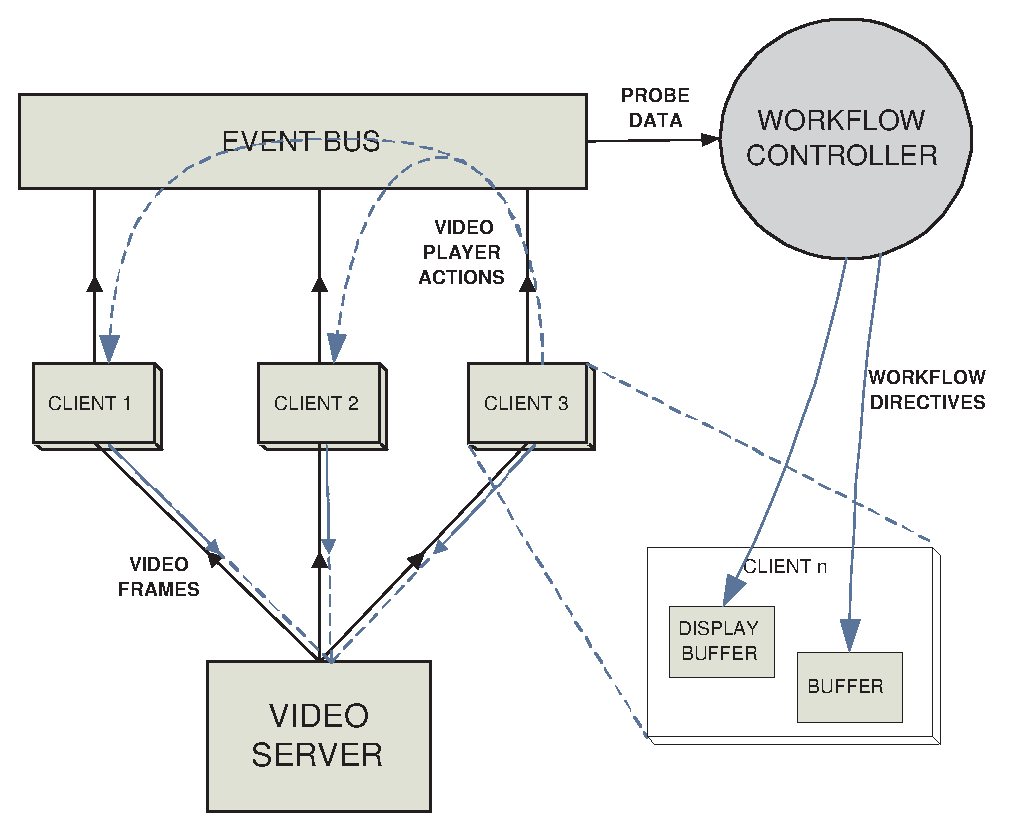
\epsfig{file=ai2tvarch.eps, width=8cm}
  \caption{$\mathrm{AI}^2$TV Architecture}
  \label{ai2tv_arch}
\end{figure}

%(FIGURE: ai2tv synchronization arch)
% video server
The video server provides the educational video content to the clients
for viewing.  The provided content has the form of an
$\mathrm{AI}^2$TV video, i.e., a hierarchy of video versions produced
by running the tool multiple times with settings for different
compression levels, which produces several sets of JPG frames that are
indexed by a frame index file.  The task of the video server is simply
to provide remote download access to the frames and the index file
over HTTP.

% video client
The task of video clients is to acquire video frames, display them at
the correct time, and provide a set of basic video functions.  Taking
a functional design perspective, the client is composed of three major
modules: a video display, a video buffer and manager for fetching and
storing downloaded frames, and a time controller.

The video display renders the JPG frames into a window for display and
provides a user interface for play, pause, goto, and stop.  When any
participant initiates one of these actions, all the other group
members receive the same command, thus all the video player actions
are synchronized.  The video display knows which frame to display by
using the current video time and display quality level to index into
the frame index for the representative frame.  Before trying to render
the frame, it asks the video buffer manager if the needed frame is
available.  The video display also includes a control entity that
enables external entities, like the autonomic controller, to adjust
the current display quality level.

The video buffer and manager constitute the downloading daemon that
continuously downloads frames at a certain level.  It keeps a hash of
the available frames and a count of the current reserve frames (frames
buffered) for each quality level.  The buffer manager also includes a
control hook that enables external entities to adjust the current
downloading quality level.

The time controller's task is to ensure that a common video clock is
maintained across clients.  It relies on NTP \cite{NTP} to synchronize
the system's software clock therefore ensuring a common time base from
which each client can reference for the video clock.  The task of each
then is to play the frames at the correct time and since all the
clients refer to the same time base, then all the clients are showing
semantically equivalent frames.

% autonomic controller
The task of the autonomic controller is to ensure that the clients
within a video session stay synchronized and that each client plays at
its highest attainable quality level.  The controller is a distributed
system, whose design derives from a conceptual reference architecture
for externalized autonomic computing platforms proposed by Kaiser
\cite{REFARCH}, which is shown in figure \ref{refarch}. The
architecture provides an end-to-end closed control loop, in which
sensors attached to a generic (possibly legacy) target system and
continuously collect and send streams of data to gauges.  The gauges
analyze the incoming data streams and respond to conditions that need
adaptation by relaying that information to controllers.  The
controllers coordinate the expression and orchestration of the
workflow needed to carry out the adaptation.  To close the loop,
actuators at the target system effect the needed adjustments under the
supervision of the controller.

%
%(figure of ref arch here). 
%

\begin{figure}
 \centering
 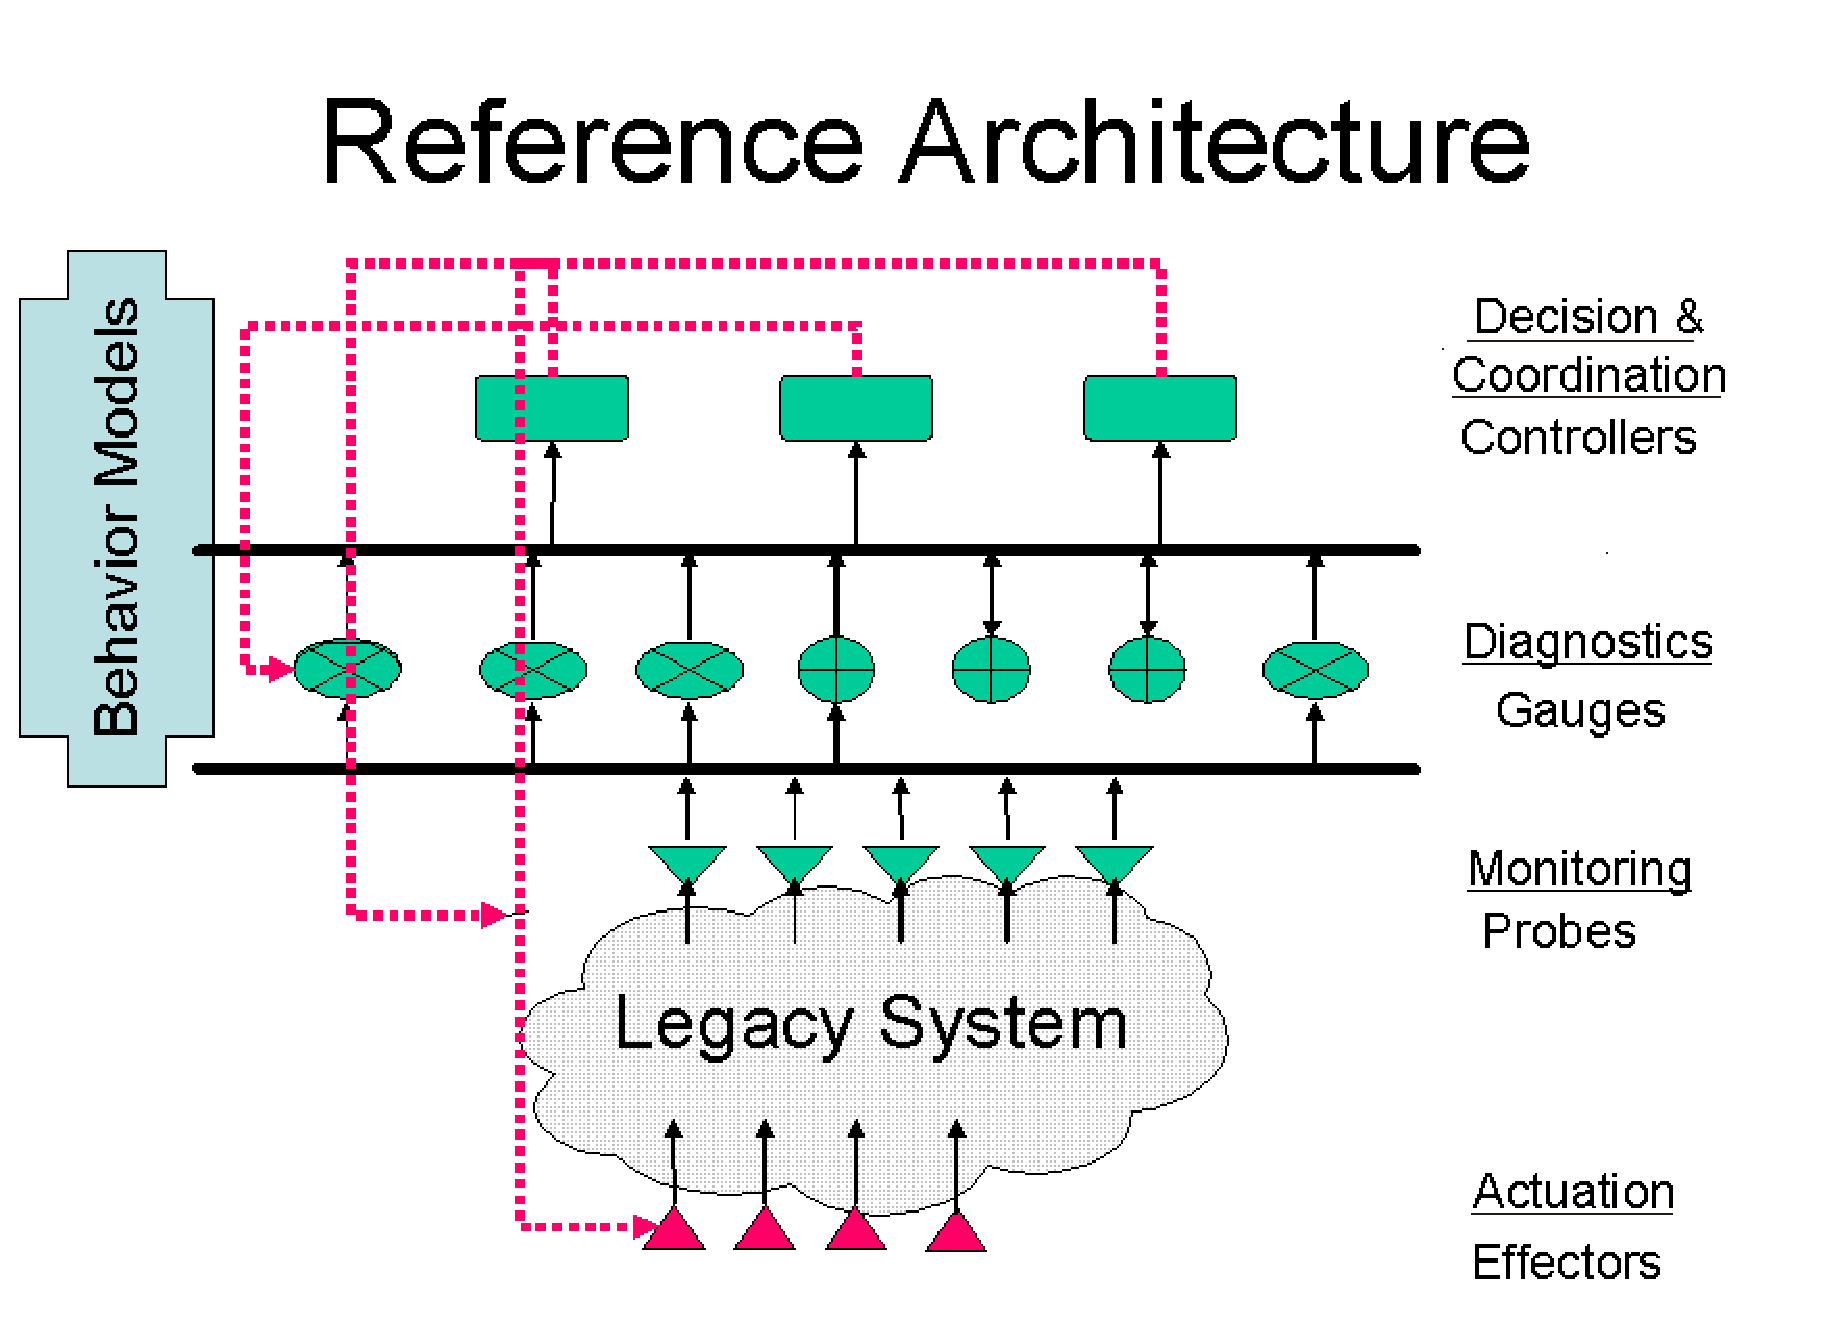
\epsfig{file=refarch.eps, width=8cm}
  \label{refarch}
 \caption{Conceptual Reference Architecture}
\end{figure}


The sensors provide the autonomic controller with data about the
clients such as video display quality level, the buffer quality level,
the buffer reserve frames, the currently displayed frame and the
current bandwidth.  Gauges are embedded together with the coordination
engine for expediency of design and to minimize the communication
latency to it.  They receive the sensor reports from individual
clients, collect them in buckets, similar to the approach in
\cite{MIMAZE}, and pass the bucket data structure to the coordination
engine.  The coordination engine directs the flow of the information
through a predefined workflow plan described in the next section.

During the evaluation of the data, a set of helper functions that are
tailored specifically for the application are used to produce the
triggers for the coordinator.  If a trigger is raised, the
coordination engine enacts an adaptation scheme which is executed on
the end hosts by hooks provided to the actuators by the end systems.

% communications 
The infrastructure used for the communications among the video
clients, as well as between the $\mathrm{AI}^2$TV system and the
autonomic controller is provided by an event bus based on the
publish/subscribe paradigm.  The reason for choosing this
communication model is that it inherently decouples the physical
location of the communicating entities.  Events transmitted onto that
event bus are of three kinds: video player actions, sensor reports and
adaptation directives (see figure \ref{ai2tv_arch}.  Video player
actions pertain to the functionality of the $\mathrm{AI}^2$TV system,
since they represent commands issued on a video client, such as pause,
play or stop, which need to be propagated to all clients in the group
to enforce the same behavior.  All video player actions are time
stamped so that clients can respond to those commands in reference to
the common time base.

\subsection{Adaptation Model}

The adaptation scheme falls into two levels: a higher level data flow,
and a lower level adjustment heuristic.  The former directs the flow
of data through a logical sequence to provide a formal decision
process while the latter provides the criteria as to when to make
certain adjustments.

The higher level logic is shown in figure \ref{ljil}, according to the
Little-JIL graphic workflow specification language \cite{LJIL}.  The
diagram shows the task decomposition hierarchy according to which the
adaptation workflow unfolds.  Note that the evaluation of clients'
state with respect to the group (\texttt{EvaluateClient}) and the
issuing of adaptation directives (\texttt{AdaptClient}) is carried out
as a set of the parallel steps.  Also note that the multiplicity of
those parallel steps is dynamically determined via the number of
entries in the \texttt{client} variable, which maps to a collection of
$\mathrm{AI}^2$TV clients.

%
%add Figure with AI2TV workflow diagram here
%

\begin{figure} 
  \centering
  \hspace*{-5mm}
  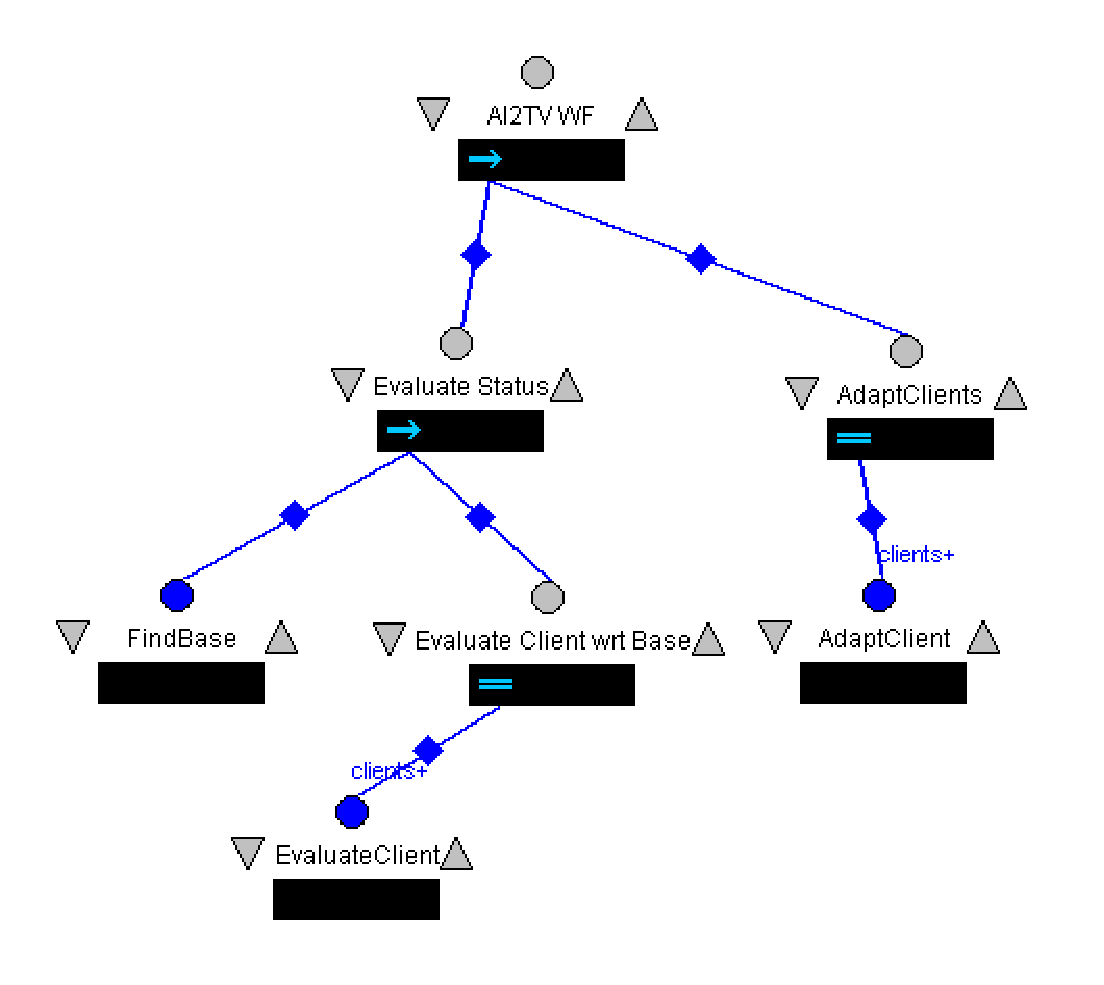
\epsfig{file=ljil.eps, width=8cm}
  \caption{$\mathrm{AI}^2$TV Workflow diagram }
  \label{ljil}
\end{figure}

The adaptation scheme at the lower level falls into two categories:
directives that adjust the client in response to relatively low
bandwidth situations, and those that take advantage of relatively high
bandwidth situations.

In the situation where a client has relatively low bandwidth, the
client may not be able download next frame at the same quality level
in time.  This situation will merit that both the client and the
buffer quality levels are reduced one level. In the case in which the
client is already at the lowest level, the controller will calculate
the next possible frame that it can successfully complete in time - in
order to remain synchronized with the rest of the team - and will ask
the client to jump ahead to that frame.

To take advantage of relatively high bandwidth situations, the buffer
manager will start to accumulate a reserve buffer.  Once the buffer
reaches a threshold value (for example, 10 buffered frames), the
autonomic controller will direct the buffer manager to start fetching
frames a higher quality level.  Once a sufficient reserve is
accumulated also at that higher level, the client is then ordered to
display frames at that quality level.  If the bandwidth drops before
the buffer manager controller can accumulate enough frames in the
higher-level reserve, then the buffer manager is dropped back down one
level.

%\section{Implementation} \label{implementation}

The video client is implemented in Java. It naively uses the
javax.swing package to render the JPG images.  The autonomic
controller, Workflakes, is also Java-based, and is built on top of the
open-source Cougaar multi-agent system \cite{COUGAAR}, which
Workflakes adapts to operate as a decentralized workflow engine.  We
used the Little-JIL graphic workflow specification language to produce
the workflow used \cite{LJIL}.  We chose a content-based
publish-subscribe event system, Siena, as our communication bus
\cite{SIENA}.

% \comment{how many lines of code?}

\section{Evaluation} \label{eval}

We assess our system by evaluating its ability to synchronize the
clients and its ability to adjust the clients video quality.  The
evaluation results presented in this section were computed from a set
of client configurations, specifically 1, 2, 3, and 5 clients running
a video for 5 minutes and probing system state every 5 seconds. The
compression hierarchy we employed has 5 different levels.

For our evaluation, we define a baseline client against which the
performance of our approach can be compared.  A baseline client is a
client whose quality level is set at the beginning of the video and
not changed thereafter.  To define the baseline client, we use a value
that we identify as the average bandwidth per level. This value is
computed by summing the total size in bytes of all frames produced at
a certain compression level and dividing by the total video time.
This value provides the bandwidth needed on average for the buffer
controller to download the next frame on time.  We provide the
baseline client with the needed bandwidth for its chosen level by
using a bandwidth throttling tool (\cite{SHAPERD}) to adjust the
bandwidth to that client from the video server.  Note that using the
average as the baseline does not account for changes in the video
frame rate and fluctuations in network bandwidth, which are situations
in which adaptive control can make a difference.

When carrying out the evaluation, each controller-assisted client is
assigned an initial level in the compression hierarchy and the same
bandwidth as the baseline client for that hierarchy level.  At the end
of each experiment, we record any differences resulting from the
adaptation of the clients' behavior on the part of the autonomic
controller and the behavior of the baseline client, with respect to
synchrony and quality of service (frame rate).

%% To evaluate our system, we produced an $\mathrm{AI}^2$TV video that had 5 quality
%% levels.  For a 17 minute video and five different window lengths, the
%% total number of frames are 165, 71, 39, 21, and 13.  Our choice of the
%% relatively low frame rate quality levels was influenced by the goal of
%% the system being used by clients with low bandwidth resources.
 
% the pathetic average frame rates (per minute!!!):
%% 3.399831413 - high
%% 1.46295776
%% 0.806289939
%% 0.434237734
%% 0.268763313 - low

\textit{Evaluating Synchrony}

A major goal of the system is to provide synchronous viewing to all
clients.  To measure the effectiveness of the synchrony, we probe the
clients at periodic time intervals and log the frame currently being
displayed.  This procedure effectively takes a snapshot of the system,
which we can evaluate for correctness.  This evaluation proceeds by
checking whether the frame being displayed at a certain time
corresponds to one of the valid frames at that time, on any arbitrary
level.  We allow any arbitrary level because the semantic compression
algorithm ensures that all frames at a certain time will contain the
same semantic information if the semantic windows overlap.  We score
the system by summing the number of clients not showing an acceptable
frame and normalizing over the total number of clients.  A score of 0
indicates a synchronized system.

Our experiments for the evaluation of synchronization initially
involved groups of clients that were set to begin playing the test
video at different levels in the compression hierarchy, and were
assigned the corresponding baseline bandwidth. In those experiments,
the results show a total score of 0 for all trials. Also,
notwithstanding the variations in the frame rate and/or occasional
fluctuations in the actual bandwidth of the clients, no frames were
missed.  This result demonstrates that the chosen baseline
combinations of compression levels and throttled bandwidths do not
push the clients beyond their bandwidth resource capacity.

We also ran another set of experiments, in which the clients in the
group were assigned more casually selected levels of starting
bandwidths.  This casual selection is representative of a real world
situation, like listening to Internet radio, where users must choose a
desired frame rate to receive.  The user may have been informed that
she is allocated a level of bandwidth from her Internet service
provider, but she may actually be receiving a significantly lower
rate.  We ran experiments first without the aid of the autonomic
controller and then with it. In the former case, clients with
insufficient bandwidth were stuck at the compression level originally
selected, and thus missed an average of 63\% of the needed frames.  In
the latter case, the same clients only missed 35\% of the needed
frames.  These results provide evidence of the benefits of the
adaptive scheme implemented by the autonomic controller.

%% selected, and thus only displayed an average of 37\% of the needed
%% frames.  In the latter case, the same clients received 65\% of the
%% needed frames.  These results provide evidence of the benefits of the
%% adaptive scheme implemented by the autonomic controller.


%% \begin{figure} 
%%   \centering
%%   \hspace*{-5mm}
%%   \epsfig{file=scores.eps, width=9cm}
%%   \caption{Comparison of weighted scores}
%%   \label{scores}
%% \end{figure}

\textit{Evaluating Quality of Service} 

A primary goal of the $\mathrm{AI}^2$TV system is to increase the
video quality for the clients.  With respect to the evaluation of
video quality of services, Liu et. al describes several local metrics
such as frame rate, loss rate, delay jitter, image resolution, and
human spatial-temporal contrast-sensitivity \cite{LIU2003}.  We do not
address global metrics such as fairness, as described in
\cite{LIU2003}.  For our situation, we focus on frame rate as a
measure of video quality.

To attain a quantitative measure of the quality of service provided by
a client assisted by the autonomic controller, we use a scoring system
relative to the baseline client's quality level.  We give a weighted
score for each level above or below the baseline quality level.  The
weighted score is calculated as the ratio of the frame rate of the two
levels.  So, for example, if a client is able to play at one level
higher then the baseline, and the baseline plays at an average
\texttt{n} fps while the level higher plays at \texttt{2*n} fps, the
given score for playing at the higher level is 2.  The weighted score
is calculated between the computed average frame rates of the chosen
quality levels.  Theoretically, the baseline client should receive a
score of 1.  Note that we formulated this scoring system because other
scoring systems \cite{BAQAI,CORTE,CONWAY2000} measure unrelated
factors such as the synchronization between different streams (audio
and video), image resolution, or human perceived quality, and are not
restricted by the group synchronization requirement.  This restriction
mandates that a scoring system be sensitive to the relative
differences between quality hierarchies.

% qos results
The evaluation of the quality of service experiments shows that the
baseline clients scored a group score of 1 (as expected) while the
clients assisted by the autonomic controller scored a group score of
1.25.  The one-tailed t-score of this difference is 3.01 which is
significant for an $\alpha$ value of .005 (N=17).  This result
demonstrates that using the autonomic controller, we are able to
achieve a significant positive difference in the quality of services.
Note that the t-score does not measure the degree of the positive
difference achieved by the autonomic controller.  To demonstrate the
degree of benefit of using the autonomic controller, we measure the
proportion of additional frames that each client maintained by the
controller is able to enjoy.  We found that overall, those clients
received 20.4\% ($\pm$ 9.7, N=17) more frames then the clients
operating at a baseline rate.

% risk assessment
The act of running the client close to or at a level higher than the
average bandwidth needed puts the client at risk for missing more
frames because the autonomic controller is trying to push the client
to a better but more resource-demanding level.  To measure whether the
controller-assisted client is exposed to a higher risk of missing
frames we also count the number of missed frames during a video
session.  The scoring of the missed frame is a simple count of the
missed frames.  Note that the scoring of the missed frame is kept
separate from the measure of the relative quality to discriminate
between levels of concern, though they both indicate a characteristic
of quality of service.

In this assessment of the risk of optimizing the frame rate, we found
that there was only one instance in which a controller-assisted client
missed two consecutive frames.  Upon closer inspection, the time
region during this event showed that the video demanded a higher frame
rate while the network bandwidth assigned to that client was
relatively low.  The client was able to consistently maintain a high
video quality level after this time.

% calculation used for the 20% number I got up there.
% baselineFrames = number of frames base client gets
% wfFrames = number of frames the wf client gets
% (wfFrames - baselineFrames) / baselineFrames = proportion of frames higher
%                                                then the baseline client

Though in some cases, using this system without the autonomic
controller may be sufficient, in most cases the network bandwidth may
vary and the variable frame rate of the video do not permit the client
to make an informed decision about the most appropriate quality level
for the next frames.  In addition, an application that does not adjust
its quality level to current bandwidth resources will not be able to
offer a level of quality appropriate to the client's resources.  To
address these issues, the autonomic controller provides an additional
adaptive element to the clients.  We show in these experiments that
the autonomic controller makes a significant positive difference in
aiding the client in achieving a higher quality level.

\section{Related Work} \label{related}
Stream synchronization is a widely studied topic in multimedia
research.  Some classifications of synchronization schemes are whether
the scheme is local or distributed (i.e., one or multiple sinks),
whether they take action reactively or pro-actively, and whether it
requires the notion of a global clock.  Our work does not deal with
the problem of inter-media synchronization of multiple modalities
(i.e., video and audio) within a multimedia stream where the concern
is to ensure the correct playback of related data originating from
different streams.  Our problem is related to intra-stream
synchronization, which is concerned with ensuring the temporal
ordering of data packets transmitted across a network from a single
streaming source to one or more delivery sinks

Most intra-stream synchronization schemes are based on data buffering
at the sink(s) and on the introduction of a delay before the play-out
of buffered data packets (i.e., frames).  Those synchronization
schemes can be rigid or adaptive \cite{Clark92}.  In rigid schemes,
such as \cite{Ferrari}, the play-out delay is chosen a priori in such
a way that it accounts for the maximum network transfer delay that can
likely occur across the sinks.  Rigid schemes work under a worst-case
scenario assumption and accept the introduction of delays that may be
longer than necessary, in order to maximize the synchronization
guarantees they can offer even in demanding situations.  

Contrary to a rigid approach, adaptive schemes \cite{ASP,Lancaster,FSP} 
recompute the delay parameter continuously while streaming: they
try to "guess" the minimum delay that can be introduced, which can
still ensure synchronization under actual operation conditions.  In
order to enhance quality of service in terms of minimized play-out
delay, those schemes must accept some temporary synchronization
inconsistencies and/or some data loss, in case the computed delay
results at times insufficient (due, for example, to variations in the
conditions of the network) and needs to be corrected on the fly.

Our approach to synchronization can be classified as a distributed
adaptive scheme that employs a global clock and operates in a
proactive way.  The main difference with respect to other approaches,
such as the Adaptive Synchronization Protocol \cite{ASP}, the work of
Gonzalez and Adbel-Wahab \cite{GONZALEZ}, or that of Liu and El
Zarki\cite{LIU} (which can all be used equally for inter- and
intra-stream applications) is that it is not based on the idea of
play-out delay.  Instead, it takes advantage of layered semantic
compression coupled with buffering to "buy more time" for clients that
might not be able to remain in sync, by putting them on a less
demanding level of the compression hierarchy.

To ensure stream synchronization across a group of clients, it is
usually necessary to implement some form of trade-off impacting the
quality of service of some of the clients.  Many schemes trade off
synchronization for longer delays, while some other approaches, like
the Concord local synchronization algorithm \cite{Concord}, allows a
choice among other quality parameters besides delay, like packet loss
rate.  Our approach sacrifices frame rates to achieve synchronization
when resources are low.

Liu et al. provide a comprehensive summary of the mechanisms used in
video multicast for quality and fairness adaptation as well as network
and coding requirements \cite{LIU}.  To frame our work in that
context, our current design models a single-rate server adaptation
scheme to each of the clients because the video quality we provide is
tailored specifically to that client's network resources.  The focus
in our work is directed towards the client side end user perceived
quality and synchrony, so we did not utilize the most efficient server
model.  The authors believe that it would be trivial to substitute in
a simulcast server adaptation model \cite{CHEUNG,LI}.  Our design also
fits into the category of layered adaptation.  This adaptation model
defines a base quality level that users must achieve.  Once users have
acquired that level, the algorithm attempts to incrementally acquire
more frames to present a higher quality video.  In the work presented
here, the definition of quality translates to a higher frame rate.
Liu's discussion of bandwidth fairness, coding techniques and network
transport perspectives lie out of the scope of this paper.

With respect to the software architecture, our approach most resembles
the Lancaster Orchestration Service \cite{Lancaster} since it is based
on a central controller that coordinates the behavior of remote
controlled units placed within the clients via appropriate directives.
(i.e., the $\mathrm{AI}^2$TV video buffer and manager).  Their
approach employs the adaptive delay-based scheme described above,
hence the playback of video focuses on adapting to the lowest
bandwidth client.  That approach would degrade the playback experience
of the other participants to accommodate the lowest bandwidth client.
Our approach differs by allowing each client to receive video quality
commensurate with its bandwidth resources.

Cen et. al provide a distributed real-time MPEG video/audio player
that uses a software feedback loop between a single server and a
single client to adjust frame rates \cite{CEN}.  Their architecture
provides the feedback logic within each video player and does not
support synchronization across a group of players, while the work
presented here provides the adaptation model within a central
controller and explicitly supports the synchronization of semantically
equivalent video frames across a group of clients.

An earlier implementation of $\mathrm{AI}^2$TV is described in
\cite{VECTORS}.  In that version, a collaborative virtual environment
(CVE) supported a variety of team interactions \cite{CHIME}, with the
optional video display embedded in the wall of a CVE ``room''.  The
same semantic compression capability was used. Video synchronization
data was piggybacked on top of the UDP peer-to-peer communication used
primarily for CVE updates, such as tracking avatar movements in the
style of multi-player 3D gaming.  The video synchronization did not
work very well, due to the heavy-weight CVE burden on local
resources. Video quality optimization was not addressed.  The new
implementation of $\mathrm{AI}^2$TV presented here can run alongside
the CVE in a separate window.

\section{Conclusion}

In this paper we present an architecture and adaptation model that
allows geographically dispersed participants to collaboratively view a
video in synchrony.  The system also employs a autonomic controller
architecture that adapts the video quality according to client network
bandwidth resources.  The other novel approach that we put present is
the use of semantic compression to facilitate the synchronization of
video content to clients with heterogeneous resources.  We rely on the
semantic compression algorithm to guarantee the semantic composition
of the video frames is equivalent for all clients.  We then distribute
appropriate versions of the video to clients according to their
current bandwidth resources.  Through the use of these tools, we hope
to close the gap between students with varying network resources to
allow collaboration to proceed in a fruitful manner.

%ACKNOWLEDGMENTS are optional
\section{Acknowledgments}
We would like to thank John Kender, Tiecheng Liu, and other members of
the High-Level Vision Lab for their assistance in using their
lecture-video semantic compression software.  We would also like to
thank the other members of the Programming Systems Lab for their
support, particularly Matias Pelenur who ported the Little-JIL
workflow notation to run on Workflakes/Cougaar.  Little-JIL was
developed by Lee Osterweil's LASER lab at the University of
Massachusetts, Amherst. Cougaar was developed by a DARPA-funded
consortium; our main Cougaar contact was Nathan Combs of BBN.
Information about the Columbia Video Network is available at
http://www.cvn.columbia.edu/. PSL is funded in part by National
Science Foundation grants CCR-0203876, EIA-0202063 and EIA-0071954,
and by Microsoft Research.

% The following two commands are all you need in the
% initial runs of your .tex file to
% produce the bibliography for the citations in your paper.
\bibliographystyle{abbrv} \bibliography{ai2tv}
% You must have a proper ".bib" file
%  and remember to run:
% latex bibtex latex latex
% to resolve all references

% ??? we'll need to do this right before submission
% \subsection{References}
% 
%% Generated by bibtex from your ~.bib file.  Run latex,
%% then bibtex, then latex twice (to resolve references)
%% to create the ~.bbl file.  Insert that ~.bbl file into
%% the .tex source file and comment out
%% the command \texttt{{\char'134}thebibliography}.

% This next section command marks the start of
% Appendix B, and does not continue the present hierarchy
%% \section{More Help for the Hardy}
%% The sig-alternate.cls file itself is chock-full of succinct
%% and helpful comments.  If you consider yourself a moderately
%% experienced to expert user of \LaTeX, you may find reading
%% it useful but please remember not to change it.

\balancecolumns % GM July 2000
% That's all folks!
\end{document}
% ---------------------------------------------------------------
% / / / / / / / / / / / / / / / / / / / / / / / / / / / / / / / /
% / / / / / / / / / / / / / / / / / / / / / / / / / / / / / / / /
% / / / / / / / / / / / / / / / / / / / / / / / / / / / / / / / /
% ---------------------------------------------------------------